\documentclass{beamer}

\usepackage[utf8x]{inputenc}
\usepackage{default}
\usetheme{Warsaw}
\usepackage{amsthm}
\usepackage{listings}
\usepackage{lstcustom}
\usepackage{multicol}
\title{Qui veut du Python ?}
\author{Anthony VEREZ (netantho@minet.net)}
\date{Décembre 2011}

%\include{pythonlisting}

\addtobeamertemplate{footline}{\insertframenumber/\inserttotalframenumber}

\lstset{showstringspaces=false,
basicstyle=\small,
numberstyle=\tiny,
numbers=left,
language=python
}


\begin{document}

\begin{frame}
\titlepage
\end{frame}

\section{Introduction}

\begin{frame}{Pourquoi Python ?}
 \begin{center}
 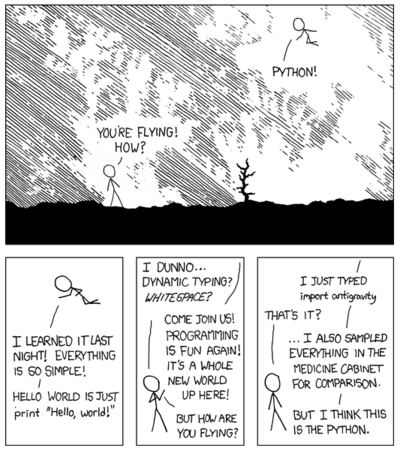
\includegraphics[scale=0.3]{./Python_cartoon.png}
 % Python_cartoon.png: 400x454 pixel, 72dpi, 14.11x16.01 cm, bb=0 0 400 454
\end{center}

\end{frame}

\begin{frame}{Quelques informations}
\begin{itemize}
 \item Langage interprété, interpréteur interactif avec la commande \textit{python}
 \item \underline{\href{http://www.tiobe.com/index.php/content/paperinfo/tpci/index.html}{8$^{\text{ème}}$ langage le plus utilisé}}
 \item Utilisé par la NASA, Google, Battlefield 2, ...
 \item Deux branches : 2.x (actuellement 2.7.2) depuis 2001 et 3.x (actuellement 3.2.2) depuis 2009. Quand ce n'est pas précisé, je vais travailler ici avec \textbf{Python 2.x}
 \item Indentation des blocs avec espaces obligatoire
 \item Librairie standard riche
 \item Programmation orienté objet
 \item Python est déjà installé sur la plupart des distributions Linux ;)
\end{itemize}
\end{frame}

\begin{frame}[fragile]{Indentation en C}{Lâchez le troll !}
\begin{lstlisting}[language=C]
#include <stdio.h>

/* Donne FALSE */
int main()
{
    if (1)
        if (0)
            printf("TRUE\n");
    else
        printf("FALSE\n");
    return 0;
}
\end{lstlisting}

\end{frame}

\begin{frame}[fragile]{Indentation en Python}{C'est mieux ! :P}
 
\begin{lstlisting}
foo = True
str = "foo"
if foo:
    if str == "bar":
        print "Bar"
    else:
        print "Foo"
    print "Foo !!!"
else:
    print "Bar !!!"
\end{lstlisting}

\end{frame}

\begin{frame}{Typage Fort}
Python est un langage à typage fort dynamique.

\begin{itemize}
 \item Les types sont déterminés à l'exécution
 \item La compilation et l'éxecution détectent les erreurs de typage
 \item Pas de conversion implicite de types, sauf un peu pour les nombres (!= PHP)
\end{itemize}

\end{frame}



\begin{frame}[fragile]{Je veux de la doc !}
\begin{itemize}
 \item \underline{\href{http://docs.python.org/}{Documentation officielle}}
 \item \underline{\href{http://diveintopython.adrahon.org/}{Plongez au c\oe{}ur de Python}}
 \item \underline{\href{http://www.afpy.org/}{AFPY Association Francophone Python}}
 \item \underline{\href{http://feldboris.alwaysdata.net/blog/pages/presentations/}{Présentation de Boris Feld, cette présentation en est inspirée}}
 \item \underline{\href{http://www.biologeek.com/bonnes-pratiques,conferences,django,python,traduction/bonnes-pratiques-et-astuces-python/}{Les bonnes pratiques}}
 \item \underline{\href{http://www.python.org/dev/peps/}{PEP Python Enhancement Proposals}}
\end{itemize}

\begin{lstlisting}
>>> help(fonction)
>>> object.__dict__
\end{lstlisting}
\end{frame}


\section{Les bases}
\begin{frame}[fragile]{Types de variables}
\begin{lstlisting}[multicols=2]
>>> type(42)
<type 'int'>
>>> type(42.) #42.==42.0
<type 'float'>
>>> type("texte")
<type 'str'>
>>> type(True)
<type 'bool'>
>>> type(0L)
<type 'long'>
>>> type(1+1j)
<type 'complex'>
\end{lstlisting}

Pas d'équivalent de \textit{char}, on n'a que des chaînes de caractères
\begin{lstlisting}
>>> type('a')
<type 'str'>
\end{lstlisting}

Conversion de types (typecasting) avec \textit{int(foo)}, \textit{str(foo)}, \dots
\end{frame}

\begin{frame}[fragile]{Chaînes de caractères}
\begin{itemize}
 \item Concaténation avec \textit{+} ou \textit{join(liste)}
\end{itemize}

\begin{lstlisting}
>>> "foo "+str(42)+" bar"
'foo 42 bar'
>>> couleurs = ['rouge', 'bleu', 'vert', 'jaune']
>>> ' '.join(couleurs) # pour liste
'rouge bleu vert jaune'
>>> x = 'string sur plusieurs \
>>> ... lignes'
>>> print x
'string sur plusieurs lignes'
>>> print "Vive\nINTech"
Vive
INTech
\end{lstlisting}
\end{frame}

\begin{frame}[fragile]{"Printf"}
\begin{lstlisting}
>>> print "%.5d euros" % (3*10)
00030 euros
>>> print "%d + %d = %d" % (2, 3, (2+3))
2 + 3 = 5
\end{lstlisting}

\end{frame}

\begin{frame}[fragile]{Opérations arithmétiques}
\begin{itemize}
 \item Opérateurs : + - * / \%
 \item Une opération sur deux nombres dans deux ensembles différents donne le résultat dans le plus "grand" (au sens de l'inclusion) ensemble
\end{itemize}

\begin{lstlisting}
>>> 2*5.
10.0
>>> 2*5j
10j
\end{lstlisting}

\end{frame}

\begin{frame}[fragile]{Affectations}
\begin{lstlisting}
>>> x = 0
>>> x
0
>>> y, z = 1, 0
>>> y
1
>>> z
0
\end{lstlisting}

\end{frame}

\begin{frame}[fragile]{Booléens}
Valeurs considérées comme fausses :
\begin{itemize}
 \item False
 \item None
 \item 0, 0.0, 0L, 0j
 \item ""
 \item (), [ ], \{ \} on en reparle ;)
\end{itemize}

\begin{lstlisting}
>>> x or y # OU logique (inclusif)
>>> x and y # ET logique
>>> not x # NON logique
\end{lstlisting}

\end{frame}


% Structures de données

\begin{frame}[fragile]{Listes}
Structure ordonnée de taille dynamique contenant une collection d'objets de types qui peuvent être différents
\begin{lstlisting}
>>> x = []
>>> type(x)
<type 'list'>
>>> x = [1, 2, 'a', 'c']
>>> x
[1, 2, 'a', 'c']
>>> x[3]
'c'
>>> list('Plop')
['P', 'l', 'o', 'p']
\end{lstlisting}

\end{frame}

\begin{frame}[fragile]{Listes - Fonctions utiles}
\begin{lstlisting}[multicols=2]
>>> x.append(5)
>>> x
[1, 2, 'a', 'c', 5]
>>> x.remove('a')
>>> x
[1, 2, 'c', 5]
>>> len(x) # taille
4
>>> l = [1, 2, 1, 1]
>>> l.count(1)
3
>>> l.count(2)
1
>>> l[1:]
[2, 1, 1]
>>> l[::-1]
[1, 1, 2, 1]
>>> # Premier indice 
>>> # d'un element
>>> l.index(1)
0
\end{lstlisting}
\end{frame}

\begin{frame}[fragile]{Tuples}
Comparables aux listes à la différence que les valeurs des tuples ne sont pas modifiables
\begin{lstlisting}[multicols=3]
>>> x = (1,2)
>>> x
(1, 2)
>>> type(x)
<type 'tuple'>
>>> x[1]
2
>>> x[:1]
(1,)
>>> x[1::2]
(2,)
>>> # pas tuple
>>> x = (1)
>>> x
1
>>> # tuple
>>> x = (1,)
>>> x
(1,)
>>> x[0]
1
>>> x[0] = 2
Traceback (most
recent call last):
File "<stdin>", 
line 1, in <module>
TypeError: 'tuple'
object does not
support item
assignment
\end{lstlisting}

\end{frame}

\begin{frame}[fragile]{Tuples - Fonctions utiles}
\begin{lstlisting}[multicols=2]
>>> l = (1, 2, 2, 3, 3, 3)
>>> l.count(2)
2
>>> l.count(3)
3
>>> l = (1, 2, 1)
>>> l.index(1)
0
>>> l.index(2)
1
>>> len(l)
3
\end{lstlisting}
\end{frame}

\begin{frame}[fragile]{Indexation négative}
\begin{lstlisting}
>>> x = [1, 2, 3, 4, 5]
>>> x[-1]
5
>>> x[-2]
4
>>> x[-5]
1
\end{lstlisting}
\end{frame}



\begin{frame}[fragile]{Dictionnaires}
Accès aux éléments non pas par des index mais par des clés (chaîne de caractères, tuple, ...), genre de "tableau associatif".\\
\begin{itemize}
 \item Clés non modifiables
 \item Structure non ordonnée
 \item Une clé pointe vers une seule valeur (qui peut néanmoins être une liste, un tuple ou un dictionnaire)
\end{itemize}
\end{frame}

\begin{frame}[fragile]{Dictionnaires}
\begin{lstlisting}
>>> positions = {}
>>> positions
{}
>>> positions = {(0,0): True, (0,1): False}
>>> positions
{(0, 1): False, (0, 0): True}
>>> positions[(0,0)]
True
>>> positions[(1,1)] = 'a'
>>> positions
{(0, 1): False, (0, 0): True, (1, 1): 'a'}
>>> positions[(0,1)] = True
>>> positions
{(0, 1): True, (0, 0): True, (1, 1): 'a'}
\end{lstlisting}
\end{frame}


\begin{frame}[fragile]{Dictionnaires - Fonctions utiles}
\begin{lstlisting}
>>> len(positions)
3
>>> positions.values()
[True, True, False]
>>> positions.keys()
[(0, 1), (0, 0), (1, 1)]
>>> del positions[(0,1)]
>>> positions
{(0, 0): True, (1, 1): 'a'}
>>> (1,1) in positions
True
\end{lstlisting}
\end{frame}


\begin{frame}[fragile]{Les itérables}
Sont itérables
\begin{itemize}
 \item Les chaînes de caractères
 \item Les tuples, listes et dictionnaires
 \item Les fichiers (sur les lignes)
\end{itemize}

\textbf{Attention}, sur les dictionnaires, les éléments itérés sont les clés alors que pour listes et tuples ce sont les valeurs

\end{frame}

\begin{frame}[fragile]{Les itérables}
\begin{lstlisting}
>>> ch = 'coucou'
>>> 'o' in ch
True
>>> map(lambda x: x+'a', ch)
['ca', 'oa', 'ua', 'ca', 'oa', 'ua']
>>> dict = {'c': 'b', 'b': 'c', 'a': 'd'}
>>> sorted(dict)
['a', 'b', 'c']
>>> sorted(dict.values())
['b', 'c', 'd']
>>> reversed(ch)
<reversed object at 0x1800a90>
>>> ''.join(list(reversed(ch))) # ne caste pas en str
'uocuoc'
\end{lstlisting}
\end{frame}

% Structures de contrôle

\begin{frame}[fragile]{Conditions}
Les opérateurs de comparaison
\begin{itemize}
 \item $==$
 \item $!=$
 \item $<=$, $>=$, $<$, $>$
\end{itemize}

\begin{lstlisting}
>>> x = 0
>>> if x > 0:
...   print "Plus grand que 0"
... elif x < 0:
...   print "Plus petit que 0"
... else:
...   print "Egal 0"
... 
Egal 0
\end{lstlisting}

On remarquera \textit{elif} et les :

\end{frame}


\begin{frame}[fragile]{Boucle for}
\begin{itemize}
 \item Sur itérable
\begin{lstlisting}[multicols=2]
>>> x = (1, 2, 3)
>>> for i in x:
...     print i
... 
1
2
3
\end{lstlisting}

 \item utilisation "Classique"
\begin{lstlisting}[multicols=2]
>>> range(5)
[0, 1, 2, 3, 4]
>>> range(2, 7)
[2, 3, 4, 5, 6]
>>> for i in range(5):
...     print i,
... 
0 1 2 3 4
>>> for i in range(5,2,-1):
...      print i,
... 
5 4 3
\end{lstlisting}

\end{itemize}

\end{frame}

\begin{frame}[fragile]{Boucle while}
\begin{lstlisting}
>>> b, i = True, 0
>>> while b:
...      print i,
...      i += 1
...      if i >= 5:
...         b = not b
... 
0 1 2 3 4
\end{lstlisting}
\end{frame}

\begin{frame}[fragile]{break et continue}
\begin{lstlisting}
>>> compteur = 0
>>> while True:
...     print compteur,
...     compteur += 1
...     if compteur >= 5:
...         break # Arrete l'execution de la boucle
...
0 1 2 3 4
>>> for x in range(10):
...     if x % 2 == 0:
...         continue # Passe au bloc suivant
...     print x
...
1 3 5 7 9
\end{lstlisting}
\end{frame}

\begin{frame}[fragile]{Entrées utilisateur}
\begin{lstlisting}
>>> s = raw_input('Vous suivez encore ? ')
Vous suivez encore ? oui
>>> s
'oui'
\end{lstlisting}

\begin{lstlisting}[language=bash]
$ echo "import sys" >> cli.py
$ echo "print sys.argv" >> cli.py
$ python cli.py INTech Powa
['cli.py', 'INTech', 'Powa']
\end{lstlisting}
\end{frame}

\begin{frame}[fragile]{Fonctions}
\begin{lstlisting}[language=python]
>>> def hello_world():
...      print "Hello World!"
... 
>>> hello_world()
Hello World!
>>> def fonction(arg1, arg2, arg3 = "val3", arg4 = "val4"):
...      return (arg1, arg2, arg3, arg4)
... 
>>> fonction("val1", "val2")
('val1', 'val2', 'val3', 'val4')
>>> fonction(arg2 = "val1", arg1 = "val2")
('val2', 'val1', 'val3', 'val4')
>>> fonction("val1", "val2", arg4 = "val1")
('val1', 'val2', 'val3', 'val1')
\end{lstlisting}
\end{frame}

\newtheorem{challenge}{Challenge}
\begin{frame}[fragile]{Démo !!!}
\begin{challenge}
Afficher les 10 derniers tweets contenant 'python' avec l'utilisateur associé et la date
\end{challenge}
\end{frame}

\begin{frame}[fragile]{Corrigé}
\begin{lstlisting}[basicstyle=\tiny]
import urllib

url = urllib.urlopen("http://search.twitter.com/search.json?q=python")

import json

monjson = json.loads(url.read())
for elem in monjson['results']:
    print elem['from_user_name']+" le "+elem['created_at']
    print elem['text']+"\n"
\end{lstlisting}

Tadam ! Rapide, non ?
\end{frame}


\begin{frame}[fragile]{Les fichiers}
\begin{lstlisting}
>>> f = open('fichier', 'w')
>>> f.write("Coucou")
>>> f.close()

>>> # Permet de fermer le fichier automatiquement 
>>> # apres traitements
>>> with open('fichier', 'r') as f:
...     print f.readlines()
['Quoi']
>>> with open('fichier', 'r') as f:
...     print f.read()
'Quoi'
\end{lstlisting}
Pour les chemins, voir le module os
\end{frame}

\section{L'orienté objet}

\begin{frame}[fragile]{Idées principales et jargon}
Un \textit{objet} en programmation est une structure de données qui contient à la fois :
\begin{itemize}
 \item Des \textit{attributs} : données sous forme de variables
  \begin{itemize}
    \item de classe : propres à une classes et communs à tous les objets de même type
    \item d'instance : propres à un objet
  \end{itemize}
 \item Des \textit{méthodes} : des moyens de traiter ces données sous forme de fonctions 
\end{itemize}
Un objet est une instance d'une \textit{classe}\\
Le \textit{constructeur} est la méthode qui est appelée à la création d'un objet
\end{frame}

\begin{frame}[fragile]{Classes}
\begin{lstlisting}
 >>> class Robot:
...   def __init__(self, couleur, roues): # constructeur
...     self.couleur = couleur # attribut d'instance
...     Robot.roues = roues # attribut de classe
...   def changerCouleur(self, couleur):
...     self.couleur = couleur
...
\end{lstlisting}
\vspace{-15px}
\begin{lstlisting}[multicols=2, numbers=none] 
>>> bot1=Robot("rouge",2)
>>> bot1.roues
2
>>> bot1.couleur
'rouge'
>>> bot1.changerCouleur("jaune")
>>> bot1.couleur
     'jaune'
     >>> bot2=Robot("bleu",3)
     >>> bot1.roues
     3
     >>> bot2.couleur
     'bleu'
\end{lstlisting}
\end{frame}

\begin{frame}[fragile]{Héritage}
\begin{lstlisting}
>>> class A:
...     a = 'A'
>>> class B:
...     b = 'B'
... 
>>> # la classe C herite des classes A et B
>>> class C(A,B):
...     pass
>>> c = C
>>> c.a
'A'
\end{lstlisting}
On peut aussi hériter de méthodes de la même façon
\end{frame}

\begin{frame}[fragile]{Surcharge d'opérateurs}
Définir les opérateurs entre des objets de même types. Il faut définir des méthodes spéciales dans les classes qui doivent retourner des booléens :
\begin{itemize}
 \item object.\_\_lt\_\_(self, b) : $a < b$
 \item object.\_\_le\_\_(self, b) : $a <= b$
 \item object.\_\_eq\_\_(self, b) : $a == b$
 \item object.\_\_ne\_\_(self, b) : a $!=$ b
 \item object.\_\_gt\_\_(self, b) : $a > b$
 \item object.\_\_ge\_\_(self, b) : $a >= b$
\end{itemize}
On a aussi des méthodes spéciales pour les opérations arithmétiques.
\end{frame}


\begin{frame}[fragile]{Modularité}
Un programme python peut s'organiser sous forme de modules.\\
Créons le module script :\\
script.py\\
\begin{lstlisting}
var = 3
def ma_fonction():
    print "ma fonction"
class C:
    pass
print "mon module"
\end{lstlisting}
Dans le même dossier, lançons l'interpréteur intéractif :
\begin{lstlisting}[basicstyle=\tiny]
>>> import script # module execute a l'importation
mon module
>>> locals()
{'__builtins__': <module '__builtin__' (built-in)>, '__name__':
'__main__', 'script': <module 'script' from 'script.py'
, '__doc__': None, '__package__': None}
\end{lstlisting}
\end{frame}

\begin{frame}[fragile]{Modularité}
Pour éviter ce genre de chose, on peut faire ça :
modularite\_execution.py
\begin{lstlisting}
print("Nom : " + __name__)
if __name__ == "__main__":
     print "Execution directe"
if __name__ == "modularite_execution":
     print "Importation"
\end{lstlisting}
\begin{lstlisting}[language=bash]
$ python modularite_execution.py 
Nom : __main__
Execution directe
\end{lstlisting}
\begin{lstlisting}
>>> import modularite_execution
Importation
\end{lstlisting}
\end{frame}

\begin{frame}[fragile]{Modularité - Packages}
On peut avoir un dossier complet pour module avec chaque fichier en sous-module.\\
Fichier obligatoire : pack/\_\_init\_\_.py
\begin{lstlisting}
print "Importation du package pack"
\end{lstlisting}
pack/test.py
\begin{lstlisting}
def f():
    print "beuh !"
\end{lstlisting}
\begin{lstlisting}
>>> import pack
Importation du package pack
>>> import pack.test
>>> pack.test.f()
beuh !
\end{lstlisting}

\end{frame}

\begin{frame}[fragile]{Modularité - Sélection fine}
Je ne veux qu'une variable, fonction ou classe
\begin{lstlisting}
>>> from pack.test import f
>>> pack
NameError: name 'pack' is not defined
>>> f
<function f at 0x7f09052ab5f0>
\end{lstlisting}
\end{frame}



\section{Les tests unitaires}

\begin{frame}[fragile]{Tests unitaires}
Un test unitaire permet de tester un programme en vérifiant générallement les retours de fonctions par rapport à des arguments données en guise de test\\
Des tests ? Pourquoi faire ?
\begin{itemize}
 \item Maîtriser sa peur de codeur en vérifiant que le programme fonctionne
 \item Connaître rapidement l'état de dégradation de son code :P
 \item Ne pas faire du refactoring à l'aveuglette
 \item Améliorer la qualité de son programme
 \item Avoir un robot qui roule le jour de la coupe :D
\end{itemize}
\end{frame}

\begin{frame}[fragile]{Nose}
Utilisation du module nose\\
\underline{\href{http://readthedocs.org/docs/nose/en/latest/}{Doc officielle (en)}}\\
\underline{\href{http://ivory.idyll.org/articles/nose-intro.html}{Didacticiel (en)}}
\begin{lstlisting}[language=bash]
$ sudo apt-get install python-nose
\end{lstlisting}
Pourquoi Nose ?
\begin{itemize}
 \item Le module \textit{unittest} existe dans la librairie standard mais il lui manque quelques fonctionnalités intéressantes
 \item Des tests qui s'écrivent facilement et rapidement dans une syntaxe python
 \item Couverture de code
 \item Configuration fine, plugins
 \item Performance : plugin pour faire du multithreadé
\end{itemize}
\end{frame}

\begin{frame}[fragile]{Utilisation basique de Nose}
demo\_tests.py
\begin{lstlisting}
import re
EMAIL_REGEX = r'[\S.]+@[\S.]+'

class testEmail:
    def test_email_regex(self):
        assert re.match(EMAIL_REGEX, 'test@mail.ru')
        assert not re.match(EMAIL_REGEX, 'test@where')
\end{lstlisting}
\end{frame}

\begin{frame}[fragile]{Utilisation basique de Nose}
\begin{lstlisting}[language=bash]
$ nosetests demo_tests.py
F
======================================================================
FAIL: demo_tests.testEmail.test_email_regex
----------------------------------------------------------------------
[...]
    assert not re.match(EMAIL_REGEX, 'test@where')
AssertionError

----------------------------------------------------------------------
Ran 1 test in 0.001s

FAILED (failures=1)
\end{lstlisting}
\end{frame}

\section{Threads}

\begin{frame}[fragile]{Téléchargeur sans threads}
\begin{lstlisting}[basicstyle=\tiny, multicols=2]
import urllib
import time

def get_file(url):
    mytime = time.ctime()
    f = urllib.urlopen(url)
    contents = f.read()
    f.close()
    print mytime+" "+url+" OK"

time_ini = time.ctime()

monurl = "http://dl.google.com/android/android-sdk_r3-linux.tgz"
for url in [monurl]*5:
     get_file(url)

print time_ini
print time.ctime()
\end{lstlisting}
\vspace{-8px}
\begin{lstlisting}[language=bash, basicstyle=\tiny]
Sun Dec 11 23:58:00 2011 http://dl.google.com/android/android-sdk_r3-linux.tgz OK
Sun Dec 11 23:58:05 2011 http://dl.google.com/android/android-sdk_r3-linux.tgz OK
Sun Dec 11 23:58:06 2011 http://dl.google.com/android/android-sdk_r3-linux.tgz OK
Sun Dec 11 23:58:08 2011 http://dl.google.com/android/android-sdk_r3-linux.tgz OK
Sun Dec 11 23:58:09 2011 http://dl.google.com/android/android-sdk_r3-linux.tgz OK
Sun Dec 11 23:58:00 2011
Sun Dec 11 23:58:11 2011
\end{lstlisting}
\end{frame}

\begin{frame}[fragile]{Téléchargeur avec threads}
\begin{lstlisting}[basicstyle=\tiny, multicols=2]
import urllib, threading
import time

class FileGetter(threading.Thread):
    def __init__(self, url):
        self.url = url
        threading.Thread.__init__(self)

    def get_result(self):
        return self.result

    def run(self):
        mytime = time.ctime()
        f = urllib.urlopen(url)
        contents = f.read()
        f.close()
        print mytime+" "+url+" OK"

time_ini = time.ctime()
tab = []
monurl = "http://dl.google.com/android/android-sdk_r3-linux.tgz"
for url in [monurl]*5:
     tab.append(FileGetter(url))
     tab[len(tab)-1].start()
for thread in tab:
     thread.join()
print time_ini
print time.ctime()
\end{lstlisting}
\begin{lstlisting}[language=bash, basicstyle=\tiny]
Sun Dec 11 23:57:56 2011 http://dl.google.com/android/android-sdk_r3-linux.tgz OK
Sun Dec 11 23:57:56 2011 http://dl.google.com/android/android-sdk_r3-linux.tgz OK
Sun Dec 11 23:57:56 2011 http://dl.google.com/android/android-sdk_r3-linux.tgz OK
Sun Dec 11 23:57:56 2011 http://dl.google.com/android/android-sdk_r3-linux.tgz OK
Sun Dec 11 23:57:56 2011 http://dl.google.com/android/android-sdk_r3-linux.tgz OK
Sun Dec 11 23:57:56 2011
Sun Dec 11 23:58:04 2011
\end{lstlisting}
\end{frame}

\begin{frame}[fragile]{Améliorations à apporter}
De nombreux d'autres problèmes sont à gérer :
\begin{itemize}
 \item Gérer l'accès concurrent à une même ressource
 \item Mettre une file d'attente (voir de priorité) pour limiter à sa guise le nombre de threads
 \item Utiliser le module multiprocessing pour faire du multi-c\oe{}urs
 \item ...
\end{itemize}
\end{frame}


\section{La liaison série}

\begin{frame}[fragile]{socat}{OMG J'émule une liaison série}
\underline{\href{http://pyserial.sourceforge.net/}{Le site officiel (en)}}
\begin{lstlisting}[language=bash]
$ sudo apt-get install socat
$ sudo apt-get install python-serial
$ socat PTY,link=./ptyp1,b9600 PTY,link=./ptyp2,b9600
\end{lstlisting}
ptyp1 et ptyp2 sont des pseudo terminaux reliés virtuellement par une liaison série.\\
\end{frame}

\begin{frame}[fragile]{Pyserial}
Ouvrir deux autres terminaux (dans le même dossier) et lancer \textit{\$ sudo python}
\begin{lstlisting}[basicstyle=\tiny, multicols=2]
>>> import serial
>>> ser = serial.Serial('./ptyp1')
>>> while 1:
...     ser.readline()
...
'INTech va tout faire peter !\n'

>>>import serial
>>>ser = serial.Serial('./ptyp2')
>>>ser.write("INTech va tout faire peter !\n")
29
\end{lstlisting}
\begin{lstlisting}[basicstyle=\tiny]
>>> # debit de Baud de 19200, timeout 1s
>>> ser = serial.Serial('./ptyp1', 19200, timeout=1)
>>> ser.read() # Lire un bit
>>> ser.read(10) # Lire 10 bits
>>> ser.close # fermer la liaison proprement
\end{lstlisting}

\end{frame}

\section{PyPy}

\begin{frame}[fragile]{Présentation de PyPy}
PyPy est une implémentation de python (2.7.1 pour l'instant) destinée à accélérer, en moyenne 3x plus vite, l'éxecution d'un programme en python (\textbf{Attention} : il faut tester au cas par cas)\\
C'est un programme python (!!) qui fait de la compilation à la volée (JIT Compilation : Just-In-Time Compilation)\\
\underline{\href{http://pypy.org/download.html}{Télécharger PyPy}}\\
Choisir "JIT Compiler" version\\
Dézipper le tout, le programme est dans pypy-1.7/bin/pypy\\
Créer un lien symbolique de pypy (avec le chemin absolu) vers /usr/bin
\end{frame}


\begin{frame}[fragile]{Pour moi qui code, quelles sont les différences ?}
\begin{itemize}
 \item lancer pypy et non python
 \item Sauf pour des extensions exotiques, persos, ... les principales fonctionnalités sont gérées à l'identique
 \item Sur ma distribution Linux, mon Mac OS X tout va bien. Sur Windows, c'est un peu moins stable.
 \item Ce qui \textbf{ne marche pas} : \small trac, Zope, Genshi, matplotlib :(, NumPy (en cours) :(, gmpy, SciPy :(, SAGE, Bazaar, Subversion, SCons, pygame :(, pyGTK, Tkinter, Cython, Pyrex, SWIG, py2exe, Fabric, Pyro
 \item Ce qui \textbf{marche} : \small Django, Pylons, Pyramid, Twisted, IPython, Scapy :), SQLAlchemy, pymongo, PyMySQL, pysqlite, redis, PIL, mechanize :), mock, nose :), Selenium Python Client Driver, unittest2
\end{itemize}
\end{frame}


\section{Python 3}

\begin{frame}[fragile]{Print}
\underline{\href{http://docs.python.org/release/3.0.1/whatsnew/3.0.html}{doc}}


\begin{lstlisting}[language=python]
>>> print "The answer is", 42 # Python 2.x
The answer is 42
>>> print("The answer is", 42) # Python 3.x
The answer is 42
>>> print(1,2) # Python 2.x
(1,2)
>>> print(1,2) # Python 3.x
1 2
\end{lstlisting}

\end{frame}

\begin{frame}[fragile]{Les Dictionnaires}
\begin{lstlisting}[language=python, multicols=2]
>>># Python 2.x
>>>dict = {(1,2): "truc"}
>>>dict.keys()
[(1, 2)]

>>> # Python 3.x
>>> dict = {(1,2): "truc"}
>>> dict.keys()
dict_keys([(1, 2)])
>>> list(dict.keys())
[(1, 2)]
\end{lstlisting}

Idem pour \textit{dict.items()}, \textit{dict.values()}
\end{frame}

\begin{frame}[fragile]{map()}
\begin{lstlisting}[language=python]
>>> # Python 2.x
>>> map(lambda x:x**2, [1,2])
[1, 4]

>>> # Python 3.x
>>> map(lambda x: x**2, [1,2])
<map object at 0x2327590>
>>> list(map(lambda x: x**2, [1,2]))
[1, 4]
\end{lstlisting}
Beaucoup d'autres changements moins importants.\\
Globalement, Python 3.x est plus orienté objet.\\
Des changements introduits dans Python 3.x sont peu à peu introduits dans Python 2.x avec rétrocompatibilité.
\end{frame}

\section{Conclusion}

\begin{frame}[fragile]{Listes compréhensives}
\begin{lstlisting}[language=python]
>>> [n ** 2 for n in range(10)]
[0, 1, 4, 9, 16, 25, 36, 49, 64, 81]
>>> [n ** 2 for n in range(10) if n % 2]
[1, 9, 25, 49, 81]
\end{lstlisting}
\end{frame}

\begin{frame}{Ce qui n'a pas été abordé}
\underline{\href{http://feldboris.alwaysdata.net/blog/pages/presentations/pythonutbm}{Voir la superbe présentation de Boris Feld}}
\begin{itemize}
 \item Gestion des exceptions
 \item Les ensembles
 \item *args et **kwargs
 \item Callbacks
 \item Fonctions anonymes/lambda (entrevu)
 \item Fonction filter
 \item Les générateurs (le robot en aura peut-être besoin, à voir)
 \item Les décorateurs
\end{itemize}
\end{frame}

\begin{frame}{Ce qui n'a pas été abordé}
Voir sur le Net ou venir me voir
\begin{itemize}
 \item Notions intermédiaires et avancée de la programmation orientée objet
 \item Gestion du verouillage, des files d'attente/de priorité pour les threads
 \item Utilisation intermédiaire et avancée de Nose
 \item Programmation avec les sockets (mais y'avait un club code dessus :P)
\end{itemize}
\end{frame}

\begin{frame}{Licence}
\begin{center}
 
\includegraphics{./88x31.png}
 % 88x31.png: 88x31 pixel, 72dpi, 3.10x1.09 cm, bb=0 0 88 31
\end{center}
\vspace{20px}
Cette oeuvre est mise à disposition selon les termes de la\\
\underline{\href{http://creativecommons.org/licenses/by-sa/3.0/}{Licence Creative Commons Paternité -}}
\underline{\href{http://creativecommons.org/licenses/by-sa/3.0/}{Partage à l'Identique 3.0 non transposé}}.

\end{frame}

\end{document}
